\section{Design Objectives \label{sec:DesignObjectives}}
The RAN-emulator which acts as load generator in both the data plane and control plane
has to satisfy the following objectives -
\begin{itemize}
	\item \textbf{High Throughput} The data plane packets should be generated at
	      a sufficient pace to saturate 40 Gbps link.
	\item \textbf{Flexible Modes} The data should be sent at a varying rate from a very low
	      load to the saturation throughput either in a single run or across different runs.
	      It should also be possible to support various modes e.g. both the data plane and control plane packets are sent together, correctness of QoS at
	      UPF can be checked, find a mapping between inter-batch delay and throughput.
	\item \textbf{Latency Measurement} The measurement of latency for both the data plane and
	      control plane packets should be possible.
	\item \textbf{Logging} The latency and throughput should be measured and logged at the
	      every fixed interval (parameter for a given run).
\end{itemize}

\section{Prior Work}
\subsection{Kernel-Based RAN}
The major limitation of this RAN is that it is not able to saturate max line rate of 40 Gbps. This is due to the fact that there are multiple copies of packet when the packet is received or transmitted - from user space to kernel space and from kernel space to the NIC buffers when the packet is forwarded.

\subsection{DPDK-based RAN}
This RAN is based on DPDK. This RAN satisfied the requirements of high data throughput and low processing latency. The current work extends on this emulator.
This emulator had satisfied most of the objectives mentioned in \ref{sec:DesignObjectives} except for the following -
\begin{itemize}
	\item Measurement of Control Plane Latency.
	\item Sending Control Plane and Data Plane Packets simultaneously.
\end{itemize}


\section{RAN Architecture}
\subsection{Threading Model}
DPDK pins one thread to each core for avoiding the overhead of context switch.
This is especially important for both the data forwarding cores and the polling
cores to get the maximum throughput per core. The auxillary threads like ARP
messages handler, heart beat messages, timers etc. can run on available free core. The cores which send data and control plane latency packets have to handle the callbacks associated with the storage of timestamps of outgoing packets. Running them on separate cores is preferred if the sufficient number of cores are available.

The NIC queues/buffers for storing the outgoing (TX-queue) and the incoming
(Rx-queue) packets are one-to one mapped to the data forwarding/polling cores.
The threads pinned to these cores process the incoming packets and prepare the packets for forwarding.


\subsection{Core Layout}
There are 24 cores on the available machines. 12 cores are available on each NUMA socket.
Although there are 2 CPUs (2 hardware threads) available on each core, hyperthreading is
kept off for reducing the non deterministic behavior attributed to contention of hardware units
and getting repeatable results.

NUMA- node 1 with starting core 12 is currently used by the RAN.
\begin{figure}[htbp]
	\centering
	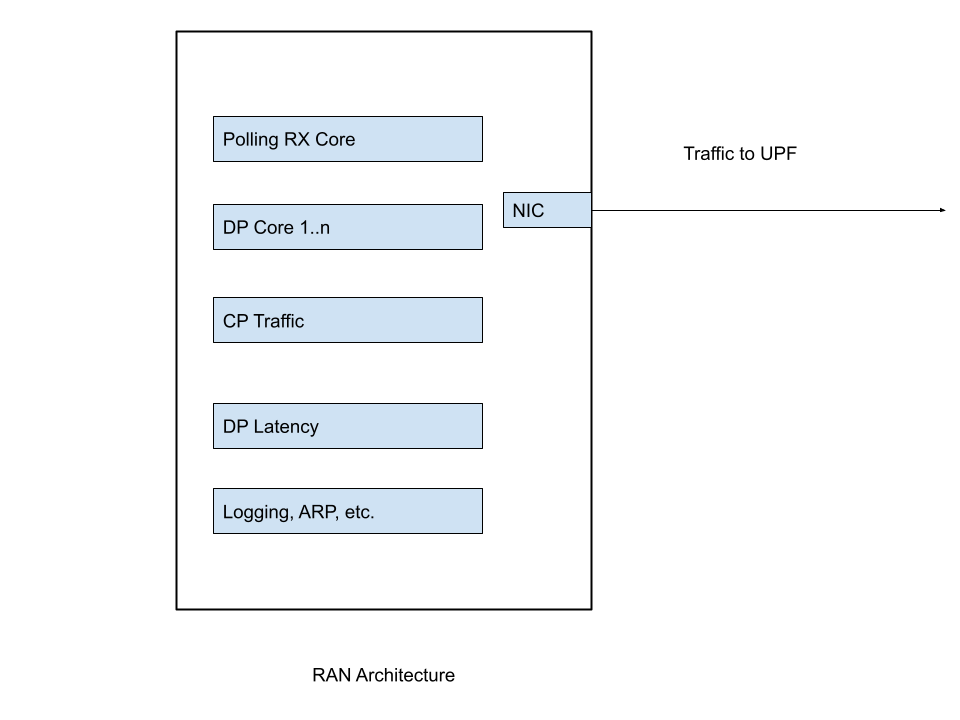
\includegraphics[width=0.8\textwidth, keepaspectratio]{./fig/Introduction/RANArchitecture.png}
	\caption{RAN Architecture}
	\label{fig:RAN}
\end{figure}

\begin{itemize}
	\item \textbf{CORE\_RX\_POLL}: Receives all the incoming packets from UPF. These includes the latency packets or data packets in the downlink direction.
	\item \textbf{CORE\_TX\_START - CORE\_TX\_END}
	      These cores are used to send data packets in the uplink  direction i.e. from RAN to UPF.
	\item \textbf{CORE\_RTT}
	      This core sends the data plane latency packets in the uplink direction. These packets are reflected back by the DNN so that end to end latency can be measured.
	\item \textbf{CORE\_CP\_TRAFFIC} This core sends the control plane traffic. A separate core was used so that a call back can be registered for storing timestamps. These timestamps are used for calculating control plane latency.
	\item \textbf{CORE\_MISC and CORE\_STAT}
	      These cores handles miscellaneous functions like ARP handling, timer and logging of stats.
\end{itemize}
Using this layout, a maximum of 7 cores are available for the data forwarding on the same numa node.
To increase this number, the functions running on CORE\_MISC and CORE\_STAT can be run parallely on the same core. Although 7 cores have been found sufficient till now to saturate 40 Gig line with 64 byte packets.

\section{Latency Calculation Mechanisms}
\subsection{Key Idea \label{subsec:KeyIdeaCPL}}
The sample packets that are used to measure latency are sent from a specific core.
When these packets are copied into a NIC buffer, a callback function is called.
This callback function stores the timestamp of the outgoing packet in an array.
The location at which the timestamp is stored is identified by anentifier
present in the outgoing packet. When the  response to a sample packet arrives
at the receiving core, a call back function is called to measure the end to
end latency or response time of the UPF. This callback function extracts the
timestamp stored previously and subtracts it from the current time to get the latency measure.

\subsection{Defintion of Control Plane Latency}
For control plane, the measured latency is the difference between two events:
\begin{itemize}
	\item Forwarding of PFCP requests - session establishment, modification, and deletion requests.
	\item Receipt of PFCP responses to the establishment, modification and response requests.
\end{itemize}
This time period includes the following major delays -
\begin{itemize}
	\item \textbf{Processing Delay} This includes the processing of request packets, updation of local data structures at UPF and preparation of response packets.
	\item \textbf{Queueing Delay} This is the time when the PFCP packets remain queued in the NIC or any userspace buffers present in the UPF and the RAN.
\end{itemize}

\subsection{Implementation Issues}
As discussed in \ref{subsec:KeyIdeaCPL}, the main issues to address for measuring control plane latency are-
\begin{enumerate}
	\item \textbf{Identify the identifier}
	      All kinds of PFCP messages have a session identifier field in Forwarding
	      Action rules that is used by the UPF to classify the data plane packets across different UEs/sessions. This field is present at different offsets for different PFCP messages. Each message is also identified by a unique number, for example - 51 for establishment request, 52 for establishment response etc. So we have  6 different kinds of messages for a given session id. A combination of both the message type and session identifier uniquely identifies the packet.
	\item \textbf{Manage the Callback Overhead} It becomes difficult to 
	process all the callbacks if the packets are sent at a sufficiently high
	 rate. The array is a performant data structure in the sense that it is
	  random access and data is stored contiguously. The access pattern in our use case an excellent spatial locality and temporal locality i.e. all the consecutive entries are accesssed one after the other (session IDs increase sequentially).
\end{enumerate}


\subsection{Details}
A fixed length array is used to store timestamps - \textbf{TSArray} . The
array size is $65536 * 3$ and stores the value of timestamp register \textbf{rdtsc} for the
outgoing packets. The first $65536$ values are used to store establishment packet related
timestamps, next $65536$ modification packet related timestamps and then release packet
timestamps are stored.  The bitwise operations can be easily used as 65536 is a power of 2.

When the corresponding response packets are received, the matching entry is retrieved from the array and latency is calculated. 

\section{Control Plane + Data Plane Traffic}

$n1$ sessions are established before the data forwarding takes place. These sessions remain established throughout the run.

$n2$ sessions are established, modified and released while the data forwarding is also taking place. The data packets are sent from all the currently established sessions. The minimum value of currently established sessions is $n1$. The maximum value is $n1+n2$.

$t1$ is the total duration of the experiment.
$t2$ is the  duration of the establishment, modification and release cycle of each of the $n2$ sessions.

The duration $t1$ for which all the static sessions $n1$ and the dynamic sessions $n2$ are used is also asked to the user.

Data forwarding starts from the $n1$ sessions at the start. After sleeping for a time (currently 5
seconds), $n2$ threads are started. The role of each thread is to sleep for a random amount of time
$t3$ ($<t2$), establish and modify the session, and then sleep for some time $t4$ and release the
session. The invariant is $t3+t4= t2$.   The session is available for data forwarding in the period $t4$.  The threads with new session Ids are started once all the previous threads have joined i.e. have finished their task.
Each of the data packet forwarding cores use all the existing established sessions/UEs to forward the data. Note that this is different from the case when sessions were partitioned among cores.

\subsection{Issues}
\begin{itemize}
	\item \textbf{Pthreads, Lthreads}
	There are two kind of threading APIs available. - Posix-threads and lthreads. Lthreads is a user level api which comes with dpdk.
	\begin{itemize}
		\item \textbf{Pthreads} This completely implemented and works correctly when locks are used in both data plane and control plane functions. 
		\item \textbf{Lthreads} DPDK has lthread API available for spawning threads on the 
		same core. This is a user space threading API with a user space scheduler. This is not preemptive and is based on cooperative scheduling -threads yield control for 
		scheduler to schedule another thread. The yielding occurs on certain points when functions like \textbf{lthread\_sleep} are called. An alternate set of control plane procedures for defining the dynamic session functionality is defined on an experimental basis. This may be used if there are performance hits in pthread implementation.
	\end{itemize}
	\item Data plane latency packets are currently sent only from first $n1$ sessions. The dynamically created sessions ($n2$) are used to send data but not the latency packets. This is not difficult to modify and technique that is used to send normal data packets can be used here as well. 

\end{itemize}
